\documentclass{article}
\usepackage[margin=1in]{geometry} 
\usepackage{amsmath,amsthm,amssymb,amsfonts, fancyhdr, color, comment, graphicx, environ}
\usepackage{xcolor}
\usepackage{mdframed}
\usepackage[utf8]{inputenc}
\usepackage[shortlabels]{enumitem}
\usepackage[obeyspaces]{url}
\usepackage{indentfirst}
\usepackage{hyperref}
\renewcommand{\footrulewidth}{0.8pt}
\usepackage{subcaption}
\usepackage{setspace}
\usepackage[
backend=biber,
style=authoryear,
]{biblatex}
\addbibresource{reference.bib} %Imports bibliography file


\parindent 2em
\parskip 1.5em

\hypersetup{
    colorlinks=true,
    linkcolor=blue,
    filecolor=magenta,      
    urlcolor=blue,
}


\pagestyle{fancy}


\lhead{The A-Team}
\rhead{CS6945 Deep Learning Capstone} 
\chead{\textbf{Final Project Report}}
\cfoot{University of Utah}


\begin{document}
\title{\Large CS6945 - Deep Learning Capstone \\[0.5cm]
        \bf\Large Final Project Report}
\author{\large Adithya Badidey, Ryan Dalby, Zhongyi Jiang\\ \ \\}
\date{\large Date Last Edited: \today}

\makeatletter
    \begin{titlepage}
        \begin{center}
	   {\ \\ \ \\}
        \vbox{}\vspace{5cm}
            {\@title }\\[3cm] 
            {\@author}
            {\@date\\}

        \end{center}
    \end{titlepage}
\makeatother%not necessary but looks fancy

\section{Introduction}
Road cracks can pose a serious safety risk for motorists, cyclists, and pedestrians on the road. 
Road cracks come in many different shapes and sizes which can indicate useful information about the state of the road. Informing transportation departments about where these cracks are can allow for maintenance crews to address them before they become a major concern.
Currently, transportation departments use a mixture of manual inspection and specialized sensing techniques (like LIDAR) to survey road conditions. 
This mapping process often only occurs every year or so because of how costly and time intensive it is.
As a result, there is a need for a real-time way to monitor road conditions to enable transportation departments to take more informed maintenance decisions and better allocate their resources. 

For our deep learning capstone project, we addressed these concerns by approaching the problem of road crack detection and size estimation using deep learning-based computer vision techniques on dashcam imagery.
Combined with the large-scale availability of real-time dashcam imagery we hope to enable the creation of real-time geospatial maps that can be dynamically updated with incoming data.

In this report, we detail methods to approach this problem including the datasets, models, and deep learning tasks involved. 
We then describe multiple crack detection and size estimation pipelines to solve this problem and specifically implement one of them.
Finally we suggest possible directions for future work and suggest improvements at each stage of the pipeline.

\section{Data Exploration}
For the crack-extraction system, the input data was Blyncsy dashcam images. 
These images vary greatly in terms of camera parameters and camera pose. Some examples of these images can be seen in Figure \ref{fig:blyncsy_dashcam_viz}
We were not provided with any ground truth crack size information. For this reason, we started to explore pre-existing datasets and how they can be used to train a model which would hopefully generalize to the Blyncsy images.

Figure \ref{fig:datasets_comparison_viz} contains a comparison of field-of-view of the different datasets we investigated for this project. Each of them contain street-level imagery and vary greatly in terms of camera perspective. This lack of standard camera parameters further complicated the task since generalizable methods mapping to the target dataset is a difficult, if not ill-posed, task without ground truth.

\begin{figure}[ht]
\begin{center}
\includegraphics[width=1\textwidth]{images/blyncsy_dashcam_viz.png}
\end{center}
\caption{Comparison of Blyncsy dashcam imagery.}
\label{fig:blyncsy_dashcam_viz}
\end{figure}


\begin{figure}[ht]
\begin{center}
\includegraphics[width=0.9\textwidth]{images/dataset_images.png}
\end{center}
\caption{Comparison of camera FOV of different datasets.}
\label{fig:datasets_comparison_viz}
\end{figure}

\subsection{RDD2020 Data}
The RDD2020 dataset was released by \cite{RDD2020} as the primary challenge of the Global Road Damage Detection Challenge 2020, which was a part of the IEEE BigData Cup 2020. The images were collected from Japan, India, and the Czech. The training dataset comprises 21041 images, and each image may contain one or more annotations in the form of bounding boxes. Each bounding box represents an instance of road damage and is labeled with one of the following four classes (additional classes in the dataset were deemed as irrelevant and discarded).
\begin{enumerate}
    \item D00: Longitudinal crack
    \item D10: Lateral linear crack
    \item D20: Alligator crack
    \item D40: Potholes
\end{enumerate}

Some training images didn't contain any road damage class (no road damage). Some examples from RDD2020 dataset can be see in Figure \ref{fig:rdd2020}.


\begin{figure}[ht]
\begin{center}
\includegraphics[width=0.8\textwidth]{images/RDD2020_annotations.png}
\end{center}
\caption{RDD2020 dataset: Some annotated examples}
\label{fig:rdd2020}
\end{figure}

\subsection{Mandli Data}
Mandli UDOT (Utah Department of Transportation) road data consists of monocular road view images of Utah state roads of constant camera parameters and pose along with associated road distress and LIDAR data.
This data is typically collected by Mandli, a private company specializing in mapping road surfaces. 
UDOT has each state road mapped at least once every year in a single direction, and every few years in both directions in a costly and time consuming process.
The mapping occurs using a specialized vehicle that is driven along the roads with a LIDAR camera and a special laser crack measurement system (\cite{pavemetricsLCMS}).
This data provides a monocular road view imagery but it is important to not the large perspective difference when compared to the input Blyncsy dashcam data as seen in Figure \ref{fig:datasets_comparison_viz}.

This data appears very useful for this project as a potential source of ground truth, but there were issues in terms of being able to programmatically access the data outside of the web interface (\cite{roadviewExplorer5}).
To overcome this, a Mandli data visualization program was created to directly be able to visualize the data for labelling given the raw folder structure the data is stored in.
This tool can be found in \verb|mandli_data_src/mandli_data_extraction.ipynb|. 
Figure \ref{fig:mandli_viz_tool} shows the Mandli data visualization tool.
This program joins the LCMS XML file with the associated monocular image and gives visual cues to that would help in labelling the data.
Unfortunately, this data was not explored more because the lack of an easy way to get large amounts of the raw folder data other than a few example folders which were used to create to tool. 
As a result, no data was manually labelled during this project although this would be the next step if the underlying data was readily accessible. 
Utilizing this data, or similar data would be very useful for being able to evaluate the crack size estimation because the LCMS data contains the needed crack size ground truth.
This data could also enable segmentation rather than instance detection through manual labelling.
Segmentation may be a better way to describe the fairly subjective measure of the where a crack starts and ends.

\begin{figure}[ht]
\begin{center}
\includegraphics[height=0.4\textwidth]{images/mandli_viz_1.png}
\includegraphics[height=0.35\textwidth]{images/mandli_viz_2.png}
\end{center}
\caption{Mandli visualization tool with two sequential images to illustrate how the monocular image corresponds to LCMS data. Note the manhole cover for reference.}
\label{fig:mandli_viz_tool}
\end{figure}

\subsection{Brazilian NDTI Dataset}
This dataset was created by \cite{Passos2020CracksAP} using data from the
Brazilian National Department of Transport Infrastructure (NDTI). These images were captured using a Highway Diagnostic Vehicle with a fixed front facing 5MP camera. The camera is installed on the highest part of the vehicle, facing the front and with an inclination closer to orthogonality. The visibility of the pavement is 15 meters. The data was developed using these images after filtering out images which present a clear view of the pavement and have some crack(s) or pothole(s). Each image in the dataset comes with 3 masks for each type of annotation: road, crack and pothole (as seen in Figure \ref{fig:brazilian_example}).


\begin{figure}[ht]
\begin{center}
\includegraphics[height=0.5\textwidth]{images/brazilian_ndti_example.png}
\end{center}
\caption{Example of the original image (a) and the masks corresponding to the road region (b), pothole (c) and crack (d).}
\label{fig:brazilian_example}
\end{figure}

This dataset provides a template for a what a good data collection method would be for use for use by deep learning methods. Since the camera is fixed, it allows makes it easier to extract meaningful information. This dataset was used to perform semantic segmentation using FCN (in subsection \ref{FCN}) and produced great results.

\subsection{KITTI Dataset}
Beyond crack data it was necessary to look at datasets which contain depth information, one of the most commonly used street level depth datasets is the KITTI dataset created by \cite{KITTI_raw_dataset}.
The KITTI dataset contains contains raw sparse LIDAR data, GPS/IMU data, and the associated color and gray-scale stereo image pairs.
This dataset can be used for a range of tasks such as depth estimation, depth completion, odometry estimation, optical flow estimation, object detection and more.

In relation to this project this dataset was leveraged for monocular depth estimation. Exploration of the dataset is shown in \verb|kitti_viz_src/kitti_data_viz.ipynb|.


\section{Methods Exploration}
To determine the crack sizes, we explored various deep learning and computer vision techniques that have been detailed in literature.
The lack of ground truth meant we had to look at individual tasks separately (each of them with their individual training data) and then join them to create a pipeline which could solve the complete task. This decision also allowed us to interpret and evaluate the results of each task separately.

First we looked at methods to find cracks within images: instance segmentation and semantic segmentation. Instance segmentation identifies each instance of a class within an image and outputs their predicted bounding box and label. Semantic segmentation tries to identify the label of each pixel in an image.

Then, we tried to estimate the size of detected cracks using various techniques such as inverse perspective transformation, monocular depth estimation, lane detection, and depth completion.  


\subsection{Instance Detection: FasterRCNN}
FasterRCNN is an object detection model proposed by \cite{NIPS2015_14bfa6bb}. FasterRCNN comes from a family of machine learning models which began with RCNN. These models work in two stages (i) region proposal; and (ii) region classifier. The first of the family, RCNN used selective search to generate region proposals and a bunch of SVM classifiers to produce classify each proposal. The second, Fast RCNN also uses selective search to generate region proposals with CNNs and a method called Region-Of-Interest Pooling (ROIPooling) to extract features for each region proposal for classification. This results in a huge speedup but the selective search algorithm was still a bottleneck.

FasterRCNN solves bottleneck of region proposal using an algorithm called Region Proposal Network (FasterRCNN has a 10x speedup over FastRCNN). Firstly, FasterRCNN uses a pre-trained CNN backbone as its first step. In case of PyTorch, the FasterRCNN comes pre-trained with  ResNet-50 and ResNet-101 backbones. The Region Proposal Network (RPN) takes the output of the backbone as input and uses a convolution to generate region proposals. These proposals are pruned using non-maximum suppression and passed on to the ROIPooling network which functions as it did in FastRCNN. There are two levels of training involved here: Training the RPN to propose regions covering objects rather than ground and training the ROIPooling to recognize the objects properly. 

Implementation details are covered further in Section \ref{FasterRCNN-Implementation}.

\subsection{Instance Detection: YOLOv5}
YOLO is a family of object detection algorithms that work by dividing images into a grid system. YOLO stands for "You Only Look Once", denoting that its a single stage detection system (unlike FasterRCNN which is a two stage system). Currently, YOLO has five generations. The latest one is YOLOv5, which is the version we used. YOLOv5 has five different variants: YOLOv5n YOLOv5s, YOLOv5m, YOLOv5l, and YOLOv5x. The only difference is the number of parameters and the complexity of the model. 

YOLOv5n is the smallest network in the YOLOv5 family. There exists a trade-off here. If the network is smaller, training and inference time will be faster. The network can handle a higher frame rate input in real-time object detection and segmentation tasks. However, its accuracy will be lower.

YOLOv5x is the largest network in the YOLOv5 family, and it is also the network we used in our project. Since, in this project, our target data is static images, we could use the relatively large model to pursue a higher accuracy. 

To train the YOLOv5 network, we must define a YML file, including all the class names. In our training dataset, each image links another label file, which provides for all the detection objects (the four corners of the boundary box and its class). Each label file contains may contain multiple rows. And each row has class name and four 2D points of the boundary boxes. We used Yolov5x as a basic model and Adam as optimizer. We trained a YOLOv5x model for 300 epochs, and the model began over-fitting after 100 epochs. It could reach the highest Precision of 0.5768 (0.5-1 score). The corresponding F1 score was 0.63. In our pipeline, we passed road images into the pre-trained YOLOv5 network. And the network will give us a few boundary boxes, which will be used for 3d projection. 
\begin{figure}[h!]
\centering
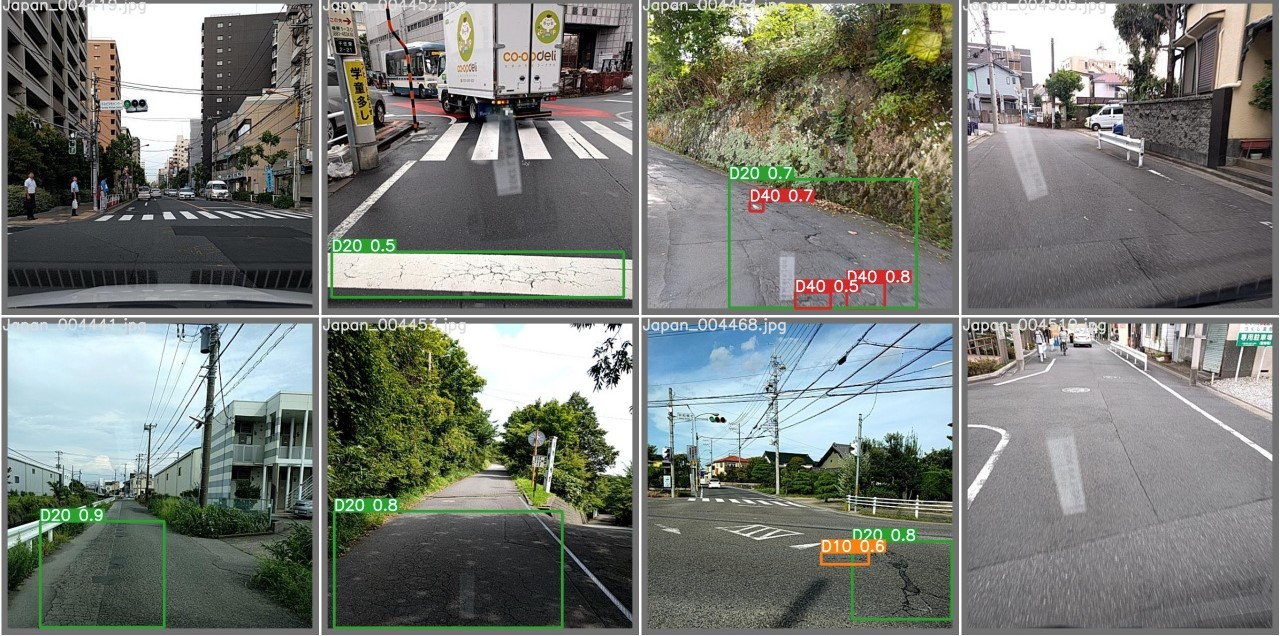
\includegraphics[width=0.9\textwidth]{images/test_batch0_pred (2).jpg}
\caption{Detection using YOLOv5 on one example in the test dataset.}
\label{fig:sample0}
\end{figure}

\subsection{Semantic Segmentation: Fully Convolutional Networks} \label{FCN}
Fully Convolutional Networks(FCN) were first proposed for use for semantic segmentation by \cite{FCNforSemanticSegmentation}. FCNs solve the problem of semantic segmentation by having the model first down-sample the image and then up-sample it to get an accurate semantic segmentation. First the image of resolution $H \times W$ is convoluted to $\frac{H}{2} \times \frac{W}{2}$ and then to $\frac{H}{4} \times \frac{W}{4}$. Then the reverse operation is done using deconvolution and adding skip-connections. Skip connections are made to allow for up-sampling using a combination of combine coarse, high layer information and fine, low layer information. The architecture seen in \ref{fig:fcnmodel} shows how three different models are created; the one we use uses a slightly different architecture which is available from PyTorch called \verb|fcn_resnet50|. It utilizes a \verb|resnet50| backbone. 

On the Brazilian NDTI Dataset, we were able to train this model to label lane, pothole and crack segments in images with a f1score of $0.60$. We used an SGD optimizer with a OneCycleLR Learning rate scheduler.  However, we found that this model did not generalize to the target Blyncsy dashcam imagery - the results were poor when the model was used on target images.

\begin{figure}[ht]
\centering
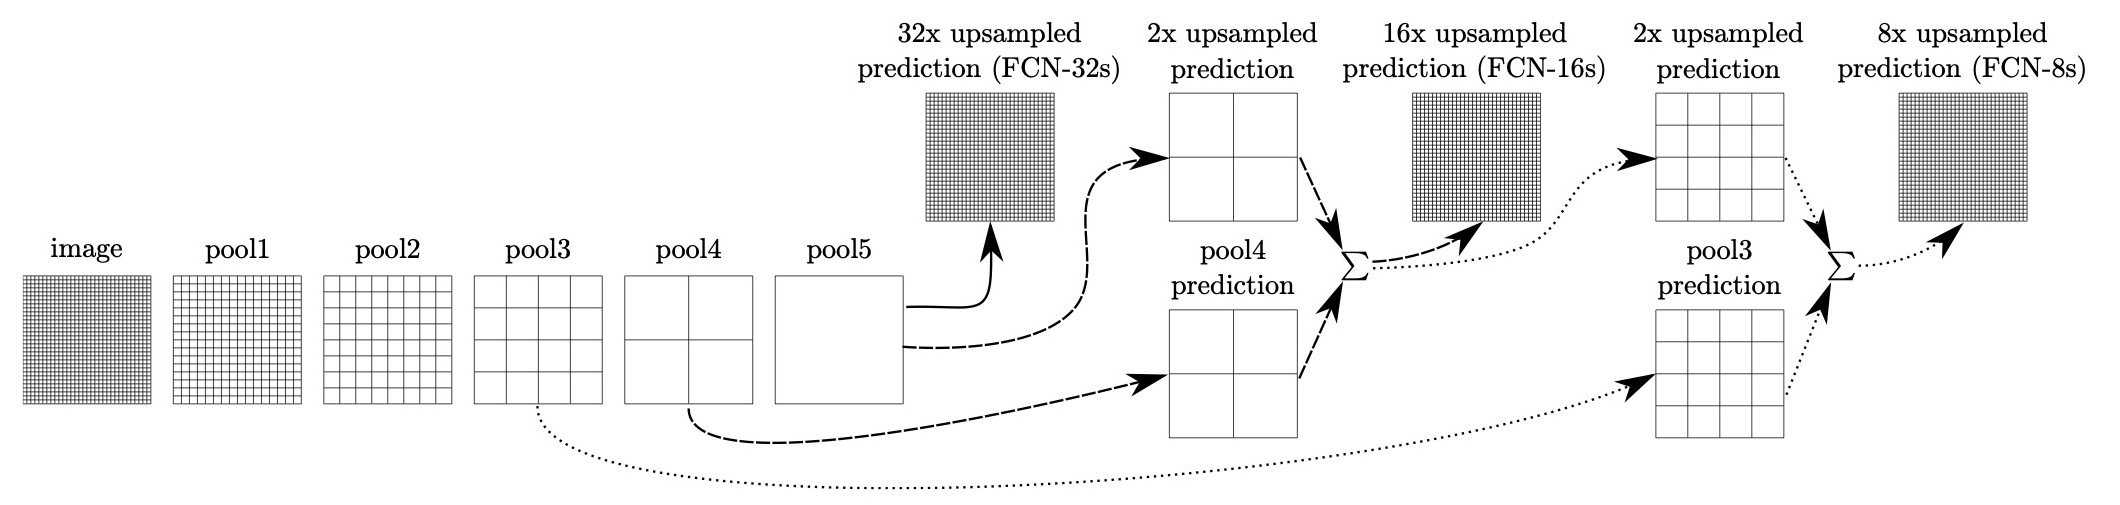
\includegraphics[width=0.9\textwidth]{images/fcn-model.jpg}
\caption{The FCN Architecture}
\label{fig:fcnmodel}
\end{figure}    

\subsection{3D Reprojection: Inverse Perspective Transformation}
For 3D reprojection, our goal is to transform any 2d coordinate in an image into a 3d coordinate in the world space. This transformation takes a 4d point (x,y,z,w), where w is the homogeneous coordinate. This perspective matrix P is $3 \times 4$ matrix (Equation \ref{matrix1})\newline

\begin{figure}[h!]
\centering
    $\begin{bmatrix}x
\\ y
\\ z

\end{bmatrix} = P(3\times4)*\begin{bmatrix}x'
\\ y'
\\ z'
\\ w'

\end{bmatrix}$

\caption{A 4D homogeneous point transformed into a 3D point by multiplying the transformation matrix P}
\label{matrix1}
\end{figure}

We can decompose the P matrix into two pieces: intrinsic Matrix and extrinsic Matrix. The camera parameters determine the intrinsic Matrix. $fx$ and $fy$ represent the focus length multiplied by the number of pixels per world unit in the x and y directions. Focus length is measured in the world unit (typically in millimeters). In the first row, the second column, there should exist a parameter s, representing the skew parameter, equal to 0. We could calculate this intrinsic Matrix through experiments. The second Matrix is called the extrinsic Matrix, and it is used to represent the coordinate transformation between the camera space and world space. The left $3\times3$ part controls the rotation, and the right $3\times1$ part controls the translation. If the camera is located at $(0,0,0)$ in the world space, we could set the left part as the identity for default and the right part as zeros (Figure\ref{P3*4}). \newline
\begin{figure}[h!]
\centering
$
\begin{bmatrix}x
\\ y
\\ z

\end{bmatrix} =\begin{bmatrix}f_{x}
 & 0 &p_{x} \\0 
 &  f_{y}& p_{y}\\0 
 &  0&1 
\end{bmatrix} *\begin{bmatrix}1
 & 0 & 0 & 0\\ 0
 & 1 &  0& 0\\ 0
 & 0 &  1& 0
\end{bmatrix} *\begin{bmatrix}x'
\\ y'
\\ z'
\\ w'

\end{bmatrix}$
\caption{Decompose the perspective matrix P into intrinsic Matrix$(3\times3)$ and extrinsic Matrix$(3\times4)$.}
\label{P3*4}
\end{figure}

So we can transfer any 3D point in camera space into a 2D point in image space. But in this project, we attempted to find the reverse corresponding (2D to 3D). To find the 3D point associated with the 2D point, we have to multiply the inverse matrix of P with the 3D vector. We used SVD decomposition to find the inverse of P and multiply it with the 2D point. But there exists a problem here. In Figure \ref{P3*4}, the z is the homogeneous coordinate. We don't know this homogeneous coordinate for reversing the process, which makes the transformation unreliable. In practice, this homogeneous coordinate is similar to the depth information. So when we do the inverse transformation, we passed in the depth estimation from the AdaBins network. Then we got the 4D (x,y,z,w) corresponding coordinate of the 2D point. We divide x, y, z by w and got the 3D point.

\begin{figure}[ht]
\centering
$\begin{bmatrix}x'
\\ y'
\\ z'
\\ w'

\end{bmatrix}=P^{-1}
\begin{bmatrix}x
\\ y
\\ z

\end{bmatrix} $
\caption{Decompose the perspective matrix P into intrinsic Matrix$(3\times3)$ and extrinsic Matrix$(3\times4)$.}
\end{figure}

\subsection{Depth Estimation: AdaBins}
A key part of this project was to estimate depth given a singular monocular image.
This is a difficult task given a single view image as depth must solely be inferred by image context. 
Traditional computer vision methods use geometry of multiple images or views of the scene using structure from motion and stereo vision matching as indicated by \cite{MonocularDepthEstimationSurvey}, these methods are not effective with a single monocular image.
Moving to deep learning methods this problem becomes approachable by leveraging LIDAR and RGB-D data from datasets such as KITTI (\cite{KITTI_raw_dataset}), NYU Depth (\cite{NYUDepth}), and more.
Supervised methods directly learn how to map from images to a depth map using loss that involves the LIDAR or RGB-D data, the architectures used follow many state-of-the-art CNN networks such as encoder-decoder and ResNet backbones. 
There is also interest in unsupervised and semi-supervised methods but these methods often require multiple sequences of images to enforce geometric constraints and learn the data distribution and suffer from scale-ambiguity as mentioned by \cite{MonocularDepthEstimationSurvey}.

For this project we had no depth ground truth or sequential images to explore these techniques, making depth estimation ill-posed.
As a result, supervised methods were pursued, with hope that in the future transfer learning using collected LIDAR or RGB-D data could overcome the inherent scale-ambiguity.

Currently, one of the state-of-the-art supervised monocular depth estimation networks is AdaBins. 
AdaBins as proposed by \cite{AdaBins} is a standard CNN encoder-decoder backbone network with an added ``AdaBins Module'' for the head of the network that aims to globally bin depths using adaptive bin sizes. 
This module utilizes a transformer to perform non-local processing of the high-level features output by the encoder-decoder, aiming to look at things in a more ``global'' way.
Pre-trained AdaBins models that were trained on the KITTI dataset and the NYU Depth dataset were available.

Given the lack of ground truth, the physical validity of AdaBins was explored using experimental techniques.
The primary question was how accurate relative distances could be, as absolute distances were expected to be inaccurate.
Multiple dashcam images were taken of a scene with a known size object and then correspondences whose difference in depth value were known were marked.
It is important to note that it was assumed, as for many parts of this project, that the depth values are relative to the camera plane, not relative to the camera location (this may be an issues for depth values in the corner of the image), often in literature it seems that this distinction is not made clear, although it can be assumed for supervised methods with a LIDAR data that the depth values are relative to the LIDAR location.
Much of the depth estimation literature does not concern itself with the physical setup of the collected data, but this can be important when it comes to practically applying one of these models and shows the necessity of things like transfer learning to bridge the difference in data.
These dashcam images were then run through pre-trained AdaBins models. 
These images were bilinearly scaled to match the input KITTI and NYU Depth dimensions then once again bilinearly scaled to match the original size.
It was found that AdaBins could get somewhat close to the actual object size values but inconsistently at best. 
It was also found that the AdaBins model pre-trained on the KITTI dataset gave more realistic results than the NYU Depth dataset, this is due to the KITTI dataset being road images while the NYU Depth dataset being primarily indoor scenes.
The results can be seen in Figure \ref{fig:ada_bins_verify}, showing that differences between the estimated and ground-truth depth differentials could be anywhere from around 0.1 meters to 10 meters or more if the chosen point was incorrectly identified as the same depth as the background.
A Jupyter Notebook of this experiment is title \verb|adabins_verify_src/adabins_verify.ipynb|.
This indicates the need to overcome the scale-ambiguity and use depth data that is directly associated with the Blyncsy input images.

\begin{figure}[ht]
\begin{center}
\includegraphics[width=0.45\textwidth]{images/adabins_verify_1.png}
\includegraphics[width=0.53\textwidth]{images/adabins_verify_2.png}
\end{center}
\caption{AdaBins physical evaluation results}
\label{fig:ada_bins_verify}
\end{figure}

\subsection{Depth Completion: PENet}
In an effort to potentially leverage the sparse Mandli LIDAR data the task of depth completion was briefly investigated. 
Currently one of the state-of-the-art depth completion networks proposed by \cite{PENet} is PENet.
This network leverages both image and sparse depth information information through two separate backbones to produce a complete depth map.
Basic usage of this network is shown in \verb|kitti_viz_src/kitti_data_viz.ipynb|.
In the future, this network could be used to accurately get full depth maps from sparse LIDAR data and monocular images. This could then be used as a better loss signal than just sparse LIDAR data for transfer learning with AdaBins.

\subsection{Lane Detection: PINet}
Lane detection using deep learning was another task that was researched.
Lacking ground truth crack information and having a scale-ambiguous problem meant that using a known size object, such as lane width would be a way to describe the width of a crack.
A near state-of-the-art network called PINet developed by \cite{PINet} was used because of its codebase being stable and developed using PyTorch with no non-Python packages needed.
This network had multiple pre-trained models available that were trained on different datasets, the one utilized for this project was trained on the TuSimple Lane dataset (\cite{tusimple}).
This network outputs estimated lane points which are classified into being part of a specific lane.
It was later found that for fitting a line to these points usage of the Hough transform worked best, this will be discussed in the pipeline section.

\section{Pipelines}

We worked towards three potential pipelines to solve this problem.

\begin{enumerate}
    \item Instance Detection model (FasterRCNN/YOLO) $\to$ AdaBins $\to$ 3d size estimation (Reprojection/Using lane width).
    
    \item Segmentation $\to$ Clustering $\to$ 3d size estimation using lane width.
    
    \item Segmentation $\to$ Clustering $\to$ AdaBins $\to$ 3d size estimation using reprojection.
\end{enumerate}

After exploring the required methods in all three pipelines for a few weeks, we realized that segmentation using FCN didnt generalize well to our target dataset and that a better dataset/model would be needed to use segmentation as part of the pipeline. Therefore, we chose to build the pipeline 1 with lane width estimation from pipeline 3 for our proof-of-concept implementation.

% We had three potential pipelines to solve this problem. We adapted the first pipeline. Firstly we used a YOLOv5 or FasterRCNN to do crack detection. We passed in road images, and the model will give us a few bounding boxes which predicted the road damages. We also applied an AdaBins model to the road image and got the depth map. The lane width estimation model will give us the width approximation. Then we used a 3D re-projection matrix to convert 2D boundary box coordinates into 3D positions and estimate the width and height of the road damage parts. The second pipeline uses segmentation and cluster to do crack detection. Then we either use 3D projection or lane width estimation to achieve the final result. All the pipelines work similarly, but we chose the first pipeline because it combines all the other methods and increases the estimation accuracy. 
\begin{figure}[ht]
\begin{center}
\includegraphics[width=\textwidth]{images/pipelines.PNG}
\end{center}
\caption{Pipeline architectures}
\label{fig:pipeline1}
\end{figure}


\section{Implemented Pipeline}
We decided to implement a proof-of-concept pipeline that could predict the bird's-eye view height and width of a crack from Blyncsy dashcam images.
The pipeline utilized crack instance detection through FasterRCNN (YOLOv5 could have also be substituted for it), depth estimation using AdaBins for both crack height estimation and width estimation using the perspective transform, and lane detection using PINet as another estimator of crack width.
This pipeline assumes on the bounding boxes tightly bounding the crack and the crack is parallel to one pair of bounding box edges, if the crack does not meet this assumption then this method may not be accurate (think a crack that goes diagonally from top right of a bounding box to the bottom left, it would be possible to recover either width or height of the crack from the bounding box dimensions but not both).

This also indicates some of the drawbacks of using bounding boxes a opposed to segmentation and also the uncertainty of what crack dimensions really mean (where a crack starts and ends can be subjective).
Thus, the task that this pipeline task hoped to achieved can be formulated as predicting the physical dimensions of the crack bounding box in world space (rather than the physical dimension of the crack).
The pipeline and all the implementation can be found in \verb|crack_size_pipeline_src/crack_size_pipeline.ipynb|.
A GeoJSON ``product'' is produced at the end of this notebook.
The product images that appear in the GeoJSON are in the form seen in Figure \ref{fig:pipeline_viz}.

\begin{figure}[ht]
\begin{center}
\includegraphics[width=0.7\textwidth]{images/pipeline_viz_1.jpeg}
\includegraphics[width=0.7\textwidth]{images/pipeline_viz_2.png}
\end{center}
\caption{Pipeline ``product" predictions.}
\label{fig:pipeline_viz}
\end{figure}

\subsection{Crack Detection} \label{FasterRCNN-Implementation}
To extract the crack's bounding boxes, we trained a FasterRCNN model using a subset of the RDD2000 Dataset (using only the Japan and Czech images). We elected to discard the India images because the road condition were very different from local Utah conditions and image quality was also subpar. 

We started with the \verb|fasterrcnn_resnet50_fpn| implementation from PyTorch, which is pre-trained on the Coco dataset. We trained this on our dataset for 5 epochs using a batch size of 32. AdamW was used as the optimizer and OneCycleLR as LRScheduler (with max a learning rate of $0.0003$. Additionally we added some random cropping, horizontal flip and color jitter to the training images to make the model generalize better. To evaluate the model, for each of the predicted bounding boxes, we checked if its a true positive or not. Using that we calculated precision and recall for each of the classes and f1-score. The best f1 score we obtained was $0.43$.

\subsection{Crack Height Estimation Using Depth}
To estimate crack height it was assumed that the depth map values were relative to a plane going through the camera. 
This meant that the difference in depth values along the detected bounding box would provide the height of the crack.
In implementation, the predicted AdaBins depth was sampled and averaged along the top and bottom edges of the bounding box, giving an averaged top and bottom depth value.
The averaged top and bottom depth values were then subtracted from each other to give a prediction of the crack height.
The error in this method could not effectively be evaluated but from the physical evaluation of AdaBins this estimate is likely not accurate and needs transfer learning to ``scale'' the depth map values correctly for the underlying data.

\subsection{Crack Width Estimation Using Inverse Perspective Transform}
The method to estimate crack width using the inverse perspective transform assumed fixed camera parameters such as focal length and camera pose.
We approximated the ``z'' homogeneous coordinate for inverse perspective transform using the AdaBins depth map and then conducted the inverse perspective transformation from image coordinates to world coordinates.
Thus the units of the AdaBins depth map determined the approximated 3D world space coordinates. 
This gave the world space coordinates of the bounding box in the same physical units as the depth map.
Then the width could be estimated as the difference in the ``x'' coordinate in 3D world space.
In the future, we could use ground-truth depth maps to calibrate the AdaBins model, use known camera parameters specific to each input image, or train a deep learning network to more generally calibrate this transformation. 

\subsection{Crack Width Estimation Using Lane Width}
The second method to estimate crack width was using lane width.
The idea of this method was that lane width could be used as a sort of high level ``ruler'' in the scene, similar to how humans use objects as visual cues to estimate sizes.
PINet was used to detect lanes, it output points representing detected lanes which were clustered into classes using a threshold.
It was found that the classification used in the published work often did not perform well enough at correctly separating unique lane lines.
Thus, clustering and linear regression techniques were explored.
These techniques did not give better results and often had issues overcoming outliers or the tight grouping of points near the horizon.

A more classical line fitting technique called the Hough transform was leveraged which robustly identifies positions of lines (and more generally shapes as described by \cite{ballard1981generalizing}).
This method works by using how points appear as sinusoids in Hough space (polar coordinate parameter space) then looking at intersection points and other properties in this space to fit lines in the original space.
This technique was able to be tuned to robustly fit lane lines to lane points as is illustrated in Figure \ref{fig:hough_transform_lane_lines}.
The Hough transform parameters are sensitive but they were tuned to be less likely to detect, this misses fitting some lines but prevent too many erratic lines.

From here predicting crack width involved looking at the average bounding box image height value and creating a heuristic which would find the width of a lane in pixels at that average height value.
Then the ratio of bounding box width in pixels to the lane width in pixels could be multiplied by the lane width's known physical dimensions to give and estimate of the crack width.

In the future, using transfer learning with Blyncsy dashcam images with labelled lane lines could further improve detection of lane lines. 
This lane detector could also find many other applications outside of crack size estimation.

\begin{figure}[ht]
\begin{center}
\includegraphics[width=0.7\textwidth]{images/hough_transform.png}
\end{center}
\caption{Utilizing the Hough transform to fit lane lines to lane points.}
\label{fig:hough_transform_lane_lines}
\end{figure}

\subsection{Discussion}
Crack height estimation relies on the accuracy of the depth estimation from AdaBins, which due to scale-ambiguity was not able to be ``calibrated'' for the input images.
The hope with this approach is that this value would be improved with future transfer learning when depth data for the dashcam images becomes available.

For crack width estimation it was found that the perspective transformation was much more robust, due it not failing when no lanes were found.
Thus to give a single width estimation, if both width estimations were found then they were averaged, or else the perspective transformation was taken. 
This weighting between these two estimation methods could be tuned in the future when ground truth is available and it is possible to determine which estimate is more accurate.
The height estimates were used directly.

Visualizing the results in \ref{fig:pipeline_viz_full} we can see cases were crack detection and crack size estimation appears to work well in terms of width estimation.
In other cases, especially those of crack misdetections the pipeline does not convey much useful information.
This also shows how in a multi-stage pipeline how errors can compound down the pipeline and why a end-to-end network would be the most flexible.

\begin{figure}[ht]
\begin{center}
\includegraphics[width=\textwidth]{images/pipeline_viz_full_1.png}
\includegraphics[width=\textwidth]{images/pipeline_viz_full_2.png}
\includegraphics[width=\textwidth]{images/pipeline_viz_full_3.png}
\includegraphics[width=\textwidth]{images/pipeline_viz_full_4.png}
\includegraphics[width=\textwidth]{images/pipeline_viz_full_5.png}
\includegraphics[width=\textwidth]{images/pipeline_viz_full_6.png}
\includegraphics[width=\textwidth]{images/pipeline_viz_full_7.png}
\end{center}
\caption{Full pipeline visualization. From left to right, crack detections with size estimates and lane lines used for size estimation, the predicted depth map, and lane line point detections with Hough transform fit linear lane lines.}
\label{fig:pipeline_viz_full}
\end{figure}

\subsection{Pipeline Evaluation}
Pipeline evaluation was not directly possible because we had no crack size ground truth so only empirical evaluation could be conducted. The crack detection algorithm itself is shown to produce good results on the target dataset.

From the results, it can be seen that the crack height estimations are not very physically accurate, for example the length of dashes in dashed lane lines is around 3 meters in the United States (\cite{us_lane_specs}).
There are many images shown in \ref{fig:pipeline_viz_full} that appear smaller in height next to dashed lane lines yet are estimated to have heights over 3 meters. 
Width estimations are much more believable because when both the perspective estimate and lane width estimate are available they are typically within a meter. 
This indicates that the errors due to the assumed camera parameters of the perspective transform are not too large, but this could not be directly confirmed.

\subsection{Future Work and Improvements}
From what we have understood implementing this proof-of-concept pipeline, we can make some suggestions as to how this can be further improved and built into a robust system.

First, crack size and depth ground truth data need to be gathered in order to truly understand how well the end-to-end pipeline is performing on the target dataset. 
There was some progress towards this during this project through using the Mandli data, but issues with having full programmatic access to the underlying data made this route difficult to pursue.
The best ground truth data would be associated with images in similar form to the input dashcam images.
This data could be collected using a LIDAR scanner, a dashcam, and a way to extract the ground truth from the LIDAR data and annotate the dashcam images with the same.
If this ground truth cannot be collected like this, then getting access to the underlying Mandli data or a similar dataset and performing manual annotation would be another route to pursue. 
Building a robust dataset like this would allow for building and training a network which can do what the pipeline is doing at a single shot.

Second, the current pipeline can be improved in a few ways. 
For instance detection, continuing training of the model with labelled crack images from the Blyncsy dashcam data would likely result in even better model performance than only using the RDD data.
For depth detection, transfer learning must be used to make AdaBins work well with the input dashcam images.
This involves collecting associated depth data for the dashcam images.
This is also crucial for an accurate inverse perspective transform.
To improve the inverse perspective transform, having known camera parameters for each dashcam image the inverse perspective transform would give a better world coordinate estimate. There seem to be some successful efforts at estimating camera parameters directly from the image by \cite{deeplearning_camera_calib}. 
Further investigation in that direction might be fruitful. 
With enough ground truth it might even be possible to use deep learning to learn an inverse perspective transform that in principle would internally estimate the camera parameters, making it have less errors than assuming a single camera model.
Lane detection could also be improved using dashcam images with labelled lane lines but using currently available methods, this seems to be less precise than the inverse perspective methods.

Third, the pipeline code needs to be ``tensorized'' to become computationally scalable.
Currently the pipeline will work with a few thousand examples in reasonable amount of time (under an hour) but this is not scalable.
Turning most operations of estimating width and height into batch tensor operations would greatly speed up inference as currently these operations a single image at a time.
The notebook code also needs to broken into modules and classes to simplify future development.

Lastly, exploring different pipelines that use instance segmentation (as opposed to object detection and semantic segmentation) to identify cracks may be a better way to identify the shape and size of cracks. This would require development of a new dataset where each crack is segmented individually. This would implementation of more accurate detection models like MaskRCNN(\cite{MaskRCNN}) and Detectron2 (\cite{wu2019detectron2}).
The inverse perspective transform too could be leveraged on a per-detected pixel basis.

\section{Conclusion}
To conclude, we were able to develop a novel crack size estimation pipeline that uses deep learning to find crack instances and infer depth information from a single dashcam image.
Due to the unavailability of ground truth, multiple publicly available datasets and pre-trained models were researched. The UDOT Mandli dataset is particularly promising but there are data accessibility issues to making this a viable option.

Many tasks that would enable this pipeline were investigated including instance detection, semantic segmentation, perspective transformation, depth detection, depth completion, and lane detection.

Depth was used as an estimator of crack height and also for crack width when combined with perspective geometry.
Crack width was also estimated using detected lanes and known lane widths.
This method was not as robust as the inverse perspective transform but has many potential applications outside of this project.
Future directions of collecting crack size data, depth data, and segmentation information can improve this pipeline and enable new ways of estimating depth.

The referenced code in this report can be found at \nolinkurl{https://github.com/UofU-CS6945/a-team-final-code}.


\section{Acknowledgements}
We would like to thank David Sacharny and Tom Henderson for their guidance and support throughout this project. This project wouldn't have been possible without Blyncsy's partnership and the computational resources they provided for exploring these deep learning methods.
We thank Arad Mohammed, Cathy Liu and Nikola Markovic for their inputs throughout the project.
And finally, we would like to thank Michael Butler with UDOT for assistance with the UDOT Mandli data.

\pagebreak 

\printbibliography

\end{document}
